\documentclass[12pt, a4paper]{report}

\usepackage[bookmarks, colorlinks=false, pdfborder={0 0 0}, pdftitle={Elevator Controller Firmware}, pdfauthor={Ghady Youssef, Antoine Karam}, pdfsubject={Elevator Controller Firmware}, pdfkeywords={Firmware design, Embedded Systems, C}]{hyperref}

\usepackage{listings}
\usepackage{graphicx}
\usepackage{xcolor}

\usepackage{amsmath}

\usepackage[
    top=3cm,
    bottom=3cm,
    left=3cm,
    right=3cm,
]{geometry}

\begin{document}

\begin{titlepage}

    \vspace*{\fill}
    \begin{center}
        \textup{\large\textbf{Firmware Design}\\
            \small{Project Report}}\\[0.3in]

        \Large \textbf {Elevator Controller}\\[0.3in]

        \begin{figure}[h]
            \centering
            
\includegraphics[width=0.65\linewidth]{assets/inci.png}
        \end{figure}

        \vspace{.5in}

        \normalsize\today\\
        Submitted by \\[0.2in]

        \textbf{Ghady Youssef}\\
        \texttt{ghady.youssef@net.usj.edu.lb}\\
        \vspace{.3in}
        \textbf{Antoine Karam}\\
        \texttt{antoine.karam3@net.usj.edu.lb}
    \end{center}
    \vspace*{\fill}

\end{titlepage}

\pagenumbering{roman}
\tableofcontents

\newpage
\pagenumbering{arabic}

\begin{abstract}
    This report presents the design and development of an elevator control system utilizing microcontrollers to manage various hardware components, including temperature sensors, real-time clocks, and motor controllers. The system's primary objectives are to optimize elevator operation through efficient scheduling, ensure safety during motor operations, and manage floor and cabin displays. The project addresses challenges such as minimizing passenger waiting times, preventing unsafe motor behavior, and ensuring reliable system performance. The integration of hardware and software components creates a robust elevator control system with potential applications in other safety-critical embedded systems.
\end{abstract}

\chapter{Introduction}

This report outlines the design and development of an elevator control system using microcontrollers to manage hardware components like temperature sensors, real-time clocks, and motor controllers. The system aims to optimize elevator operations by implementing an efficient scheduling algorithm, ensuring safety during motor operations, and managing floor and cabin displays.

The project addresses many challenges, including minimizing passenger waiting times and preventing unsafe motor behavior. It integrates hardware components with software interfaces and real-time scheduling algorithms, creating a reliable and efficient system for elevator operation.

\chapter{Firmware Architecture}

\begin{figure}[ht]
    \centering
    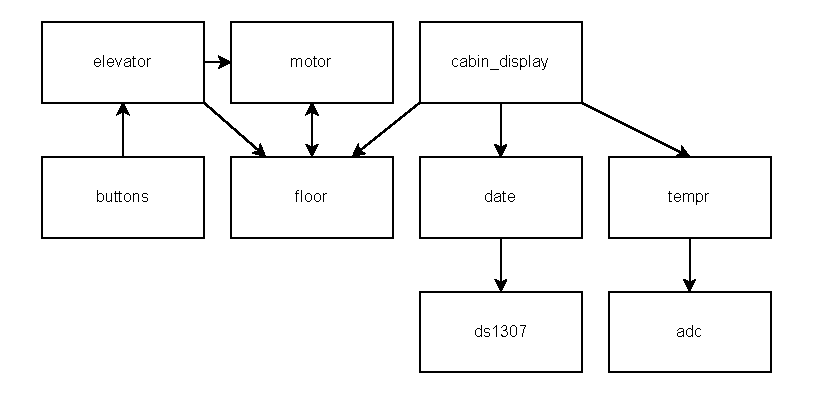
\includegraphics[width=\textwidth]{assets/block-diagram.pdf}
    \caption{Block diagram representing the firmware architecture}
\end{figure}

\chapter{Drivers}

\section{Temperature: LM35}

The \textbf{LM35} is a temperature sensor used to display the temperature inside the cabin. Its implementation is straightforward, as it has already been implemented in another project. The LM35 is connected to the system's analog-to-digital converter (ADC), utilizing the ADC driver.

The temperature API provides two main functions: one to directly get the temperature and another to get it in BCD format, allowing easy display on the cabin's 7-segment displays, limited to 2 digits.

\section{Real-Time Clock: DS1307}

In order to display the date and time inside the cabin, we used the \textbf{DS1307} Real-Time Clock. We referred to the datasheet to implement the required driver code, exposing a \texttt{read\_reg} function to read from the internal chip registers. The \texttt{date} API contains utility functions which allows us to retrieve the date, month, year and time data.
The driver code was implemented using I$^2$C, in order to transfer the regitser data from the chip to the microcontroller.

\chapter{Display}

\section{Floor Display}

The floor displays on each floor and inside the cabin show the current status of the cabin's floor. The \texttt{floor} API monitors through the \texttt{floor\_state\_monitor} task the swtiches present on each floor and updates the \texttt{current\_floor} global state. The current state can be accessed through the \texttt{get\_current\_floor} function.

\section{Cabin Display}

The cabin display shows the time (HH:MM), date (DD MM), and current temperature (TT °C) in sequence, cycling every 10 seconds. It utilizes four 7-segment displays, paired with a separator display in the middle.

The temperature is retrieved in BCD format using the temperature API, while the time and date are fetched from the data API, also in BCD format, facilitating the display on the 7 segments.

The cabin display operates as a low-priority task running every 1 second. This frequency ensures the display separator blinks in a heartbeat-like manner when showing the time and allows timely updates from the APIs in case of any changes.

\chapter{Motor}

The motor is a crucial component of the elevator system, responsible for moving the cabin between floors.

\section{Motor Operations}

The motor API provides two main functions. One function is used by the elevator scheduler, which is discussed in the next section, and another to determine the motor's current direction. The motor direction is important for both the scheduler and the floor display, as it helps the scheduler choose the next floor and it ensures the correct arrow is shown for the cabin's movement.

The motor determines its movement based on the current floor provided by the floor api and the target floor provided by the scheduler. It listens to the switches to manage speed: it accelerates when leaving the start floor, decelerates as it approaches the destination, and stops once it reaches the target.

\section{Safety Considerations}

The motor is designed with passenger safety in mind, ensuring that it does not blindly follow scheduler commands that could lead to unsafe behavior.

A key safety feature prevents the motor from suddenly changing direction. If the motor is already moving in one direction and the scheduler requests a change to the opposite direction, the motor will ignore the new request until it reaches its current destination and becomes idle. This ensures that the motor does not perform abrupt or unsafe directional changes, maintaining a safe ride.

In cases where the scheduler reschedules the motor to a new floor in the same direction, the motor will accept new the scheduler request. This design ensures a balance between responsiveness and safety.

\chapter{Scheduler}

\section{Responsibility}

The scheduler's primary responsibility is to determine the next floor the elevator should move to based on the current position, the direction of the motor, and the floor and cabin requests. It ensures that the elevator operates efficiently by selecting the most optimal floor to serve, maximizing resource utilization given that there is only one elevator in the system.

Additionally, the scheduler is responsible for ensuring safe operation by avoiding abrupt direction changes. It prevents selecting a new floor that requires a sudden shift in direction, ensuring predictable elevator movement for the safety of the passengers.

The elevator scheduler processes incoming requests from the cabin and from each floor. It selects the next target floor for the elevator, taking into account priorites, and staying in the same direction, while minimizing long trips if possible.

To manage these requests, the scheduler stores two queues: one for requests to go up and another for requests to go down.

\section{Elementary algorithm}
\begin{enumerate}
    \item When the elevator is \textbf{completely} idle, it is free to go in any direction.
    \item When the elevator is going in a direction, it must preserve this direction until the respective queues becomes empty.
\end{enumerate}

\section{Reordering the queues}
When we reach the destination (the top of the queue) and dequeue it, we have to reorder both queues to ensure the invariant of the \texttt{queue\_t}'s first and second are preserved. That is, the first part contains the floors which are \textit{(resp. below, above)} the current floor for the \textit{(resp. down, up)} queues and the second part contains the floors which are \textit{(resp. above, below)} the cabin floor for the \textit{(resp. down, up)} queue.

\begin{figure}[ht]
    \centering
    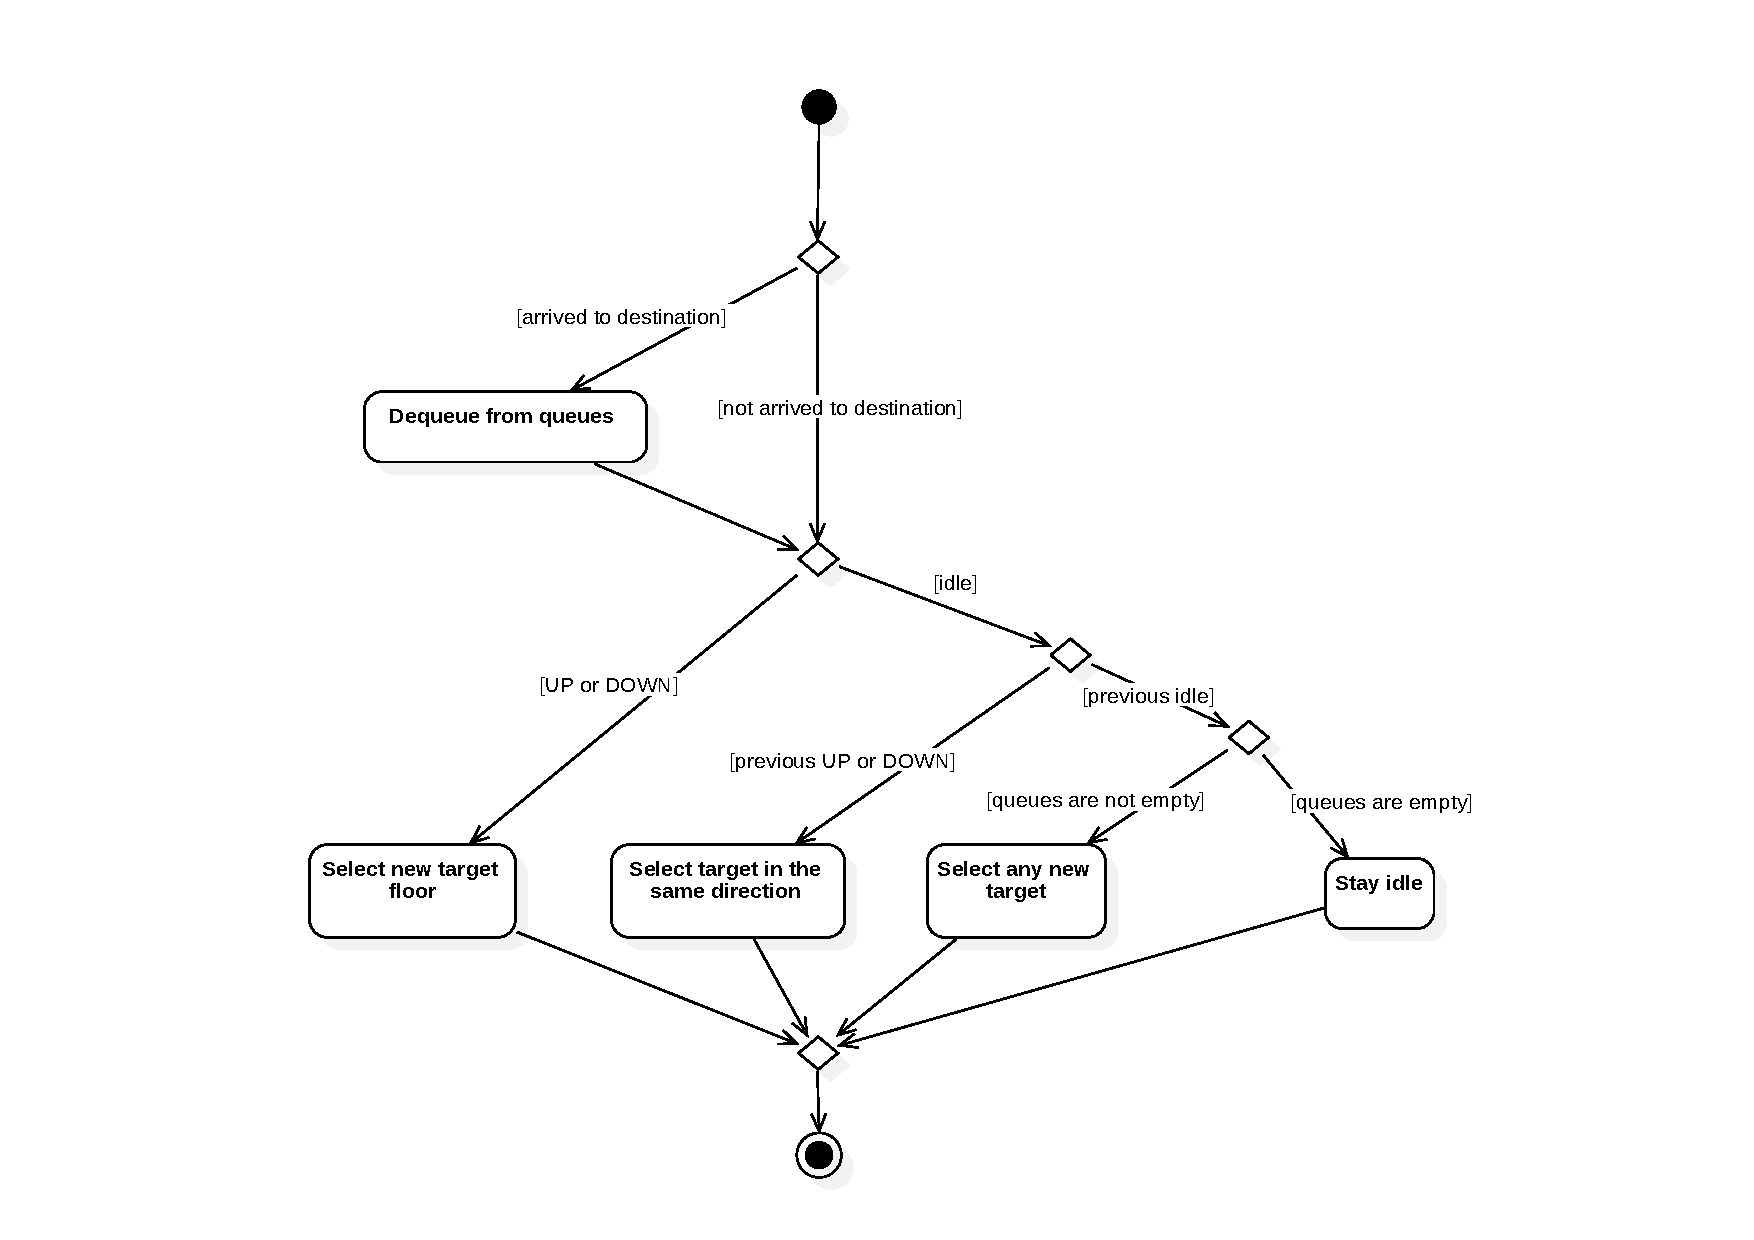
\includegraphics[width=\textwidth]{assets/scheduler.pdf}
    \caption{Activity diagram showcasing the elevator scheduling algorithm}
\end{figure}

\chapter{Development Workflow}

\section{Version Control}

To complete this project, we made great use of developer tools like Git. It allowed us to easily collaborate and distribute the tasks between the team members. We also heavily relied on GitHub Issues to assign tasks to each of the team members. When each issue is completed a pull request is created by the assignee and reviewed by the other member to ensure that both members are aware of the changes made to the codebase. This was a great opportunity to practice modern software engineering methodologies.

We seperated our work into feature (or fix) branches which were constantly created from the \texttt{dev} branch. Once each feature is completed, it is then merged back into main. We primarily use \texttt{dev} for our workflow while \texttt{main} acts as a mirror of \texttt{dev} to push new releases.

\section{Continuous Integration (CI)}

To ensure the codebase remains clean and free of unnecessary style issues, we used \texttt{clang-format} with a specific configuration to keep the styling consistent. Additionally, we used \texttt{cppcheck} to check for any additional linting warnings or errors that we could have missed during development.

Furthermore, we developed CI pipelines using GitHub Actions in order to automate building releases, style checks, and generate documentation using \texttt{doxygen}. Since most off the codebase already contains comments in the \texttt{doxygen} format, it made complete sense to have a pipeline dedicated for generating documentation. The live documentation is a available at \href{https://ghaadyy.github.io/elevator-controller/}{https://ghaadyy.github.io/elevator-controller/}.

\chapter{Challenges}

One of the core challenges faced during the development of this project was to effectively design the elevator's scheduling algorithm. We wanted to create an efficient algorithm that maximizes the number of trips in the same direction.

We had to thouroughly test and debug in order to make sure the algorithm works \textit{correctly}. When we were in doubt during the development, we made great use of the debugger to step through the code. Most of the time, the errors were logical and not related to the compilation of the code itself. Moreover, we decided to work on the elevator scheduler in a pair-programming fashion. Since this was a difficult task, reasoning throughout this problem together allowed us to progress much faster.

Every time we solve a bug, another one arises, and we have to carefully analyze and document every possible interaction the scheduler might encounter. This helps us process all edge cases and ensure a reliable scheduler. Throughout this process, we've had to revise the elevator design multiple times. Initially, we stored all requests in a single queue, but we then switched to using separate queues for external and internal requests. Later, we merged the cabin and floor requests into two queues, one for requests to go up and another for requests to go down. Eventually, we divided these queues into two parts to further optimize the process.

\chapter{Future Work}

\section{Error Detection}

Currently, there is no mechanism in place to anticipate what might happen if the power suddenly fails or if the motor stops unexpectedly. We need to implement error detection and handling procedures to address these potential failures, ensuring a safe ride for passengers under all circumstances.

\end{document}